\documentclass{sigchi}

% Use this section to set the ACM copyright statement (e.g. for
% preprints).  Consult the conference website for the camera-ready
% copyright statement.

% Copyright
\CopyrightYear{2016}
%\setcopyright{acmcopyright}
\setcopyright{acmlicensed}
%\setcopyright{rightsretained}
%\setcopyright{usgov}
%\setcopyright{usgovmixed}
%\setcopyright{cagov}
%\setcopyright{cagovmixed}
% DOI
\doi{http://dx.doi.org/10.475/123_4}
% ISBN
\isbn{123-4567-24-567/08/06}
%Conference
\conferenceinfo{CHI'16,}{May 07--12, 2016, San Jose, CA, USA}
%Price
\acmPrice{\$15.00}

% Use this command to override the default ACM copyright statement
% (e.g. for preprints).  Consult the conference website for the
% camera-ready copyright statement.

%% HOW TO OVERRIDE THE DEFAULT COPYRIGHT STRIP --
%% Please note you need to make sure the copy for your specific
%% license is used here!
% \toappear{
% Permission to make digital or hard copies of all or part of this work
% for personal or classroom use is granted without fee provided that
% copies are not made or distributed for profit or commercial advantage
% and that copies bear this notice and the full citation on the first
% page. Copyrights for components of this work owned by others than ACM
% must be honored. Abstracting with credit is permitted. To copy
% otherwise, or republish, to post on servers or to redistribute to
% lists, requires prior specific permission and/or a fee. Request
% permissions from \href{mailto:Permissions@acm.org}{Permissions@acm.org}. \\
% \emph{CHI '16},  May 07--12, 2016, San Jose, CA, USA \\
% ACM xxx-x-xxxx-xxxx-x/xx/xx\ldots \$15.00 \\
% DOI: \url{http://dx.doi.org/xx.xxxx/xxxxxxx.xxxxxxx}
% }

% Arabic page numbers for submission.  Remove this line to eliminate
% page numbers for the camera ready copy
% \pagenumbering{arabic}

% Load basic packages
\usepackage{balance}       % to better equalize the last page
\usepackage{graphics}      % for EPS, load graphicx instead 
\usepackage[T1]{fontenc}   % for umlauts and other diaeresis
\usepackage{txfonts}
\usepackage{mathptmx}
\usepackage[pdflang={en-US},pdftex]{hyperref}
\usepackage{color}
\usepackage{booktabs}
\usepackage{textcomp}

%graphic packages
\usepackage{subfigure}
%\usepackage{float}

% Some optional stuff you might like/need.
\usepackage{microtype}        % Improved Tracking and Kerning
% \usepackage[all]{hypcap}    % Fixes bug in hyperref caption linking
\usepackage{ccicons}          % Cite your images correctly!
% \usepackage[utf8]{inputenc} % for a UTF8 editor only

% If you want to use todo notes, marginpars etc. during creation of
% your draft document, you have to enable the "chi_draft" option for
% the document class. To do this, change the very first line to:
% "\documentclass[chi_draft]{sigchi}". You can then place todo notes
% by using the "\todo{...}"  command. Make sure to disable the draft
% option again before submitting your final document.
\usepackage{todonotes}

% Paper metadata (use plain text, for PDF inclusion and later
% re-using, if desired).  Use \emtpyauthor when submitting for review
% so you remain anonymous.
\def\plaintitle{Investigating Hand-Size and Mobile Touch Interactions}
\def\plainauthor{First Author, Second Author, Third Author,
  Fourth Author, Fifth Author, Sixth Author}
\def\emptyauthor{}
\def\plainkeywords{Authors' choice; of terms; separated; by
  semicolons; include commas, within terms only; required.}
\def\plaingeneralterms{Documentation, Standardization}

% llt: Define a global style for URLs, rather that the default one
\makeatletter
\def\url@leostyle{%
  \@ifundefined{selectfont}{
    \def\UrlFont{\sf}
  }{
    \def\UrlFont{\small\bf\ttfamily}
  }}
\makeatother
\urlstyle{leo}

% To make various LaTeX processors do the right thing with page size.
\def\pprw{8.5in}
\def\pprh{11in}
\special{papersize=\pprw,\pprh}
\setlength{\paperwidth}{\pprw}
\setlength{\paperheight}{\pprh}
\setlength{\pdfpagewidth}{\pprw}
\setlength{\pdfpageheight}{\pprh}

% Make sure hyperref comes last of your loaded packages, to give it a
% fighting chance of not being over-written, since its job is to
% redefine many LaTeX commands.
\definecolor{linkColor}{RGB}{6,125,233}
\hypersetup{%
  pdftitle={\plaintitle},
% Use \plainauthor for final version.
%  pdfauthor={\plainauthor},
  pdfauthor={\emptyauthor},
  pdfkeywords={\plainkeywords},
  pdfdisplaydoctitle=true, % For Accessibility
  bookmarksnumbered,
  pdfstartview={FitH},
  colorlinks,
  citecolor=black,
  filecolor=black,
  linkcolor=black,
  urlcolor=linkColor,
  breaklinks=true,
  hypertexnames=false
}

% create a shortcut to typeset table headings
% \newcommand\tabhead[1]{\small\textbf{#1}}

% End of preamble. Here it comes the document.
\begin{document}

\title{\plaintitle}

\numberofauthors{3}
\author{%
  \alignauthor{Iris Figalist\\
    \affaddr{Ludwig-Maximilians-Universit{\"a}t}\\
    \affaddr{Munich, Germany}\\
    \email{I.Figalist@campus.lmu.de}}\\
  \alignauthor{Jonas Mattes\\
    \affaddr{Ludwig-Maximilians-Universit{\"a}t}\\
    \affaddr{Munich, Germany}\\
    \email{J.Mattes@campus.lmu.de}}\\
  \alignauthor{Sarah Prange\\
    \affaddr{Ludwig-Maximilians-Universit{\"a}t}\\
    \affaddr{Munich, Germany}\\
    \email{Sarah.Prange@campus.lmu.de}}\\
}

\maketitle

\begin{abstract}
  UPDATED---\today. This sample paper describes the formatting
  requirements for SIGCHI conference proceedings, and offers
  recommendations on writing for the worldwide SIGCHI
  readership. Please review this document even if you have submitted
  to SIGCHI conferences before, as some format details have changed
  relative to previous years. Abstracts should be about 150 words and
  are required.
\end{abstract}

\category{H.5.m.}{Information Interfaces and Presentation
  (e.g. HCI)}{Miscellaneous} \category{See
  \url{http://acm.org/about/class/1998/} for the full list of ACM
  classifiers. This section is required.}{}{}

\keywords{\plainkeywords}

------------------Sarah ----------------------------------
\section{Introduction}
% part and parcel of everyday life
Interaction with your personal mobile device is an individual daily routine. Devices are increasingly smart and have plenty of functions. As today's mobile devices vary highly in their dimensions, interaction has different levels of difficulties. One or two hands might be necessary for different tasks.\\
People have different hand sizes and tend to have different device sizes, although that might not be closely interlinked. Mobile touch interactions differ widely with hand and device size.\\
Besides mobility, personalization is an important aspect. Our smartphone can only be smart based on our personal information, like for example our residence, contacts and browsing habits. Our hand size could be another personalization aspect and make our devices even smarter. If my device knows about my hand size, it could for instance adapt the layout to help us reaching the important interaction elements.\\
The paper is organized as follows. We start with an overview of related work. What has been investigated a lot so far is the touch behavior of different users. An example is touch precision in relation in to the user's hand size. In our study, we were aiming at finding the backward conclusion from the user's touch input to his hand size. We present our study design and procedure before showing our results. We conclude with a discussion and an outlook to future work.

------------------Iris ----------------------------------
\section{Related Work}
Parhi et al. performed a study about the error rates and preferred positions of different sized targets on a screen. They found out that as the target's size increases the error rate and time to reach decreases. Users also preferred the middle of the screen in contrast to the upper left and lower right corner \cite{parhi2006target}. Another study by Karlson et al. also demonstrates that the middle of the screen is the easiest to reach for a user while reaching the corners is more time consuming \cite{karlson2006studies}. Buschek and Alt also took the hand size into consideration and discovered that users with smaller hands show a larger y-offset in the upper left corner but are more accurate in the lower area of the screen when trying to hit a target \cite{buschek2015touchml}.  Bergstrom et al. defined a functional area which is the reachable region of a user's thumb without repositioning his hand. Smaller hands also show a lesser functional area \cite{bergstrom2014modeling}. As observed by Boring et al. users reposition their hand in order to reach certain areas of the screen \cite{boring2012fat}. 

\section{Study}
In order to find correlations between a user's hand size and his mobile touch interactions we implemented an android application to measure data for different interactions. 

\subsection{Study Design}
Since we wanted the measured data to be as natural as possible we chose to investigate four main gestures which users have to perform regularly when operating a smartphone: tapping, swiping, scrolling and zooming. The latter was tested in two tasks which concludes in five tasks in total. The user was allowed to adapt his hand position while performing these tasks. At the beginning of our exploratory study it was unclear whether this natural behaviour could deliver any useful results at all. This is why we chose to add a sixth unnatural task for which the hand position was predetermined. The radius of the user's thumb was meausured while he was holding the phone next to the heel of the hand. The specific tasks were designed as followed:
\begin{itemize}
	\item{Radius task:} The user was supposed to swipe a quarter circle from the right edge of the screen to the lower left
	\item{Tapping task:} The user was instructed to hit small crosses on the screen as pecisely as possible. 144 crosses appeared in an randomized order
	\item{Scrolling task:} The user had to scroll a list from top to bottom
	\item{Swiping task:} The user was supposed to swipe a slider from left to right. Four slider positions were tested: top, middle, bottom and diagonal
	\item{Maximum zooming task:} The user had to zoom a blue rectangle as far as possible with one zoom gesture
	\item{Frame zooming task:} The user was instructed to zoom a blue rectangle to fit into a frame. Three frame sizes were tested: small, medium and large. The user was allowed to execute multiple zoom gestures
\end{itemize}The phone we used for our study was the HTC one max with a screen size of 5.9 inches. The study design was within subjects so all participants performed all of the tasks. The first one always was the unnatural interaction followed by the rest in an randomized order. It was also neccessary to measure the participants' hands in order to compare the hand sizes to the measured data delivered by our application. We chose to measure the participants' hand length, width, total span (from thumb to pinky finger) and zooming span (from thumb to index finger) in order to have more options for possible correlations. 

\begin{figure*}
	\subfigure[Total Span]{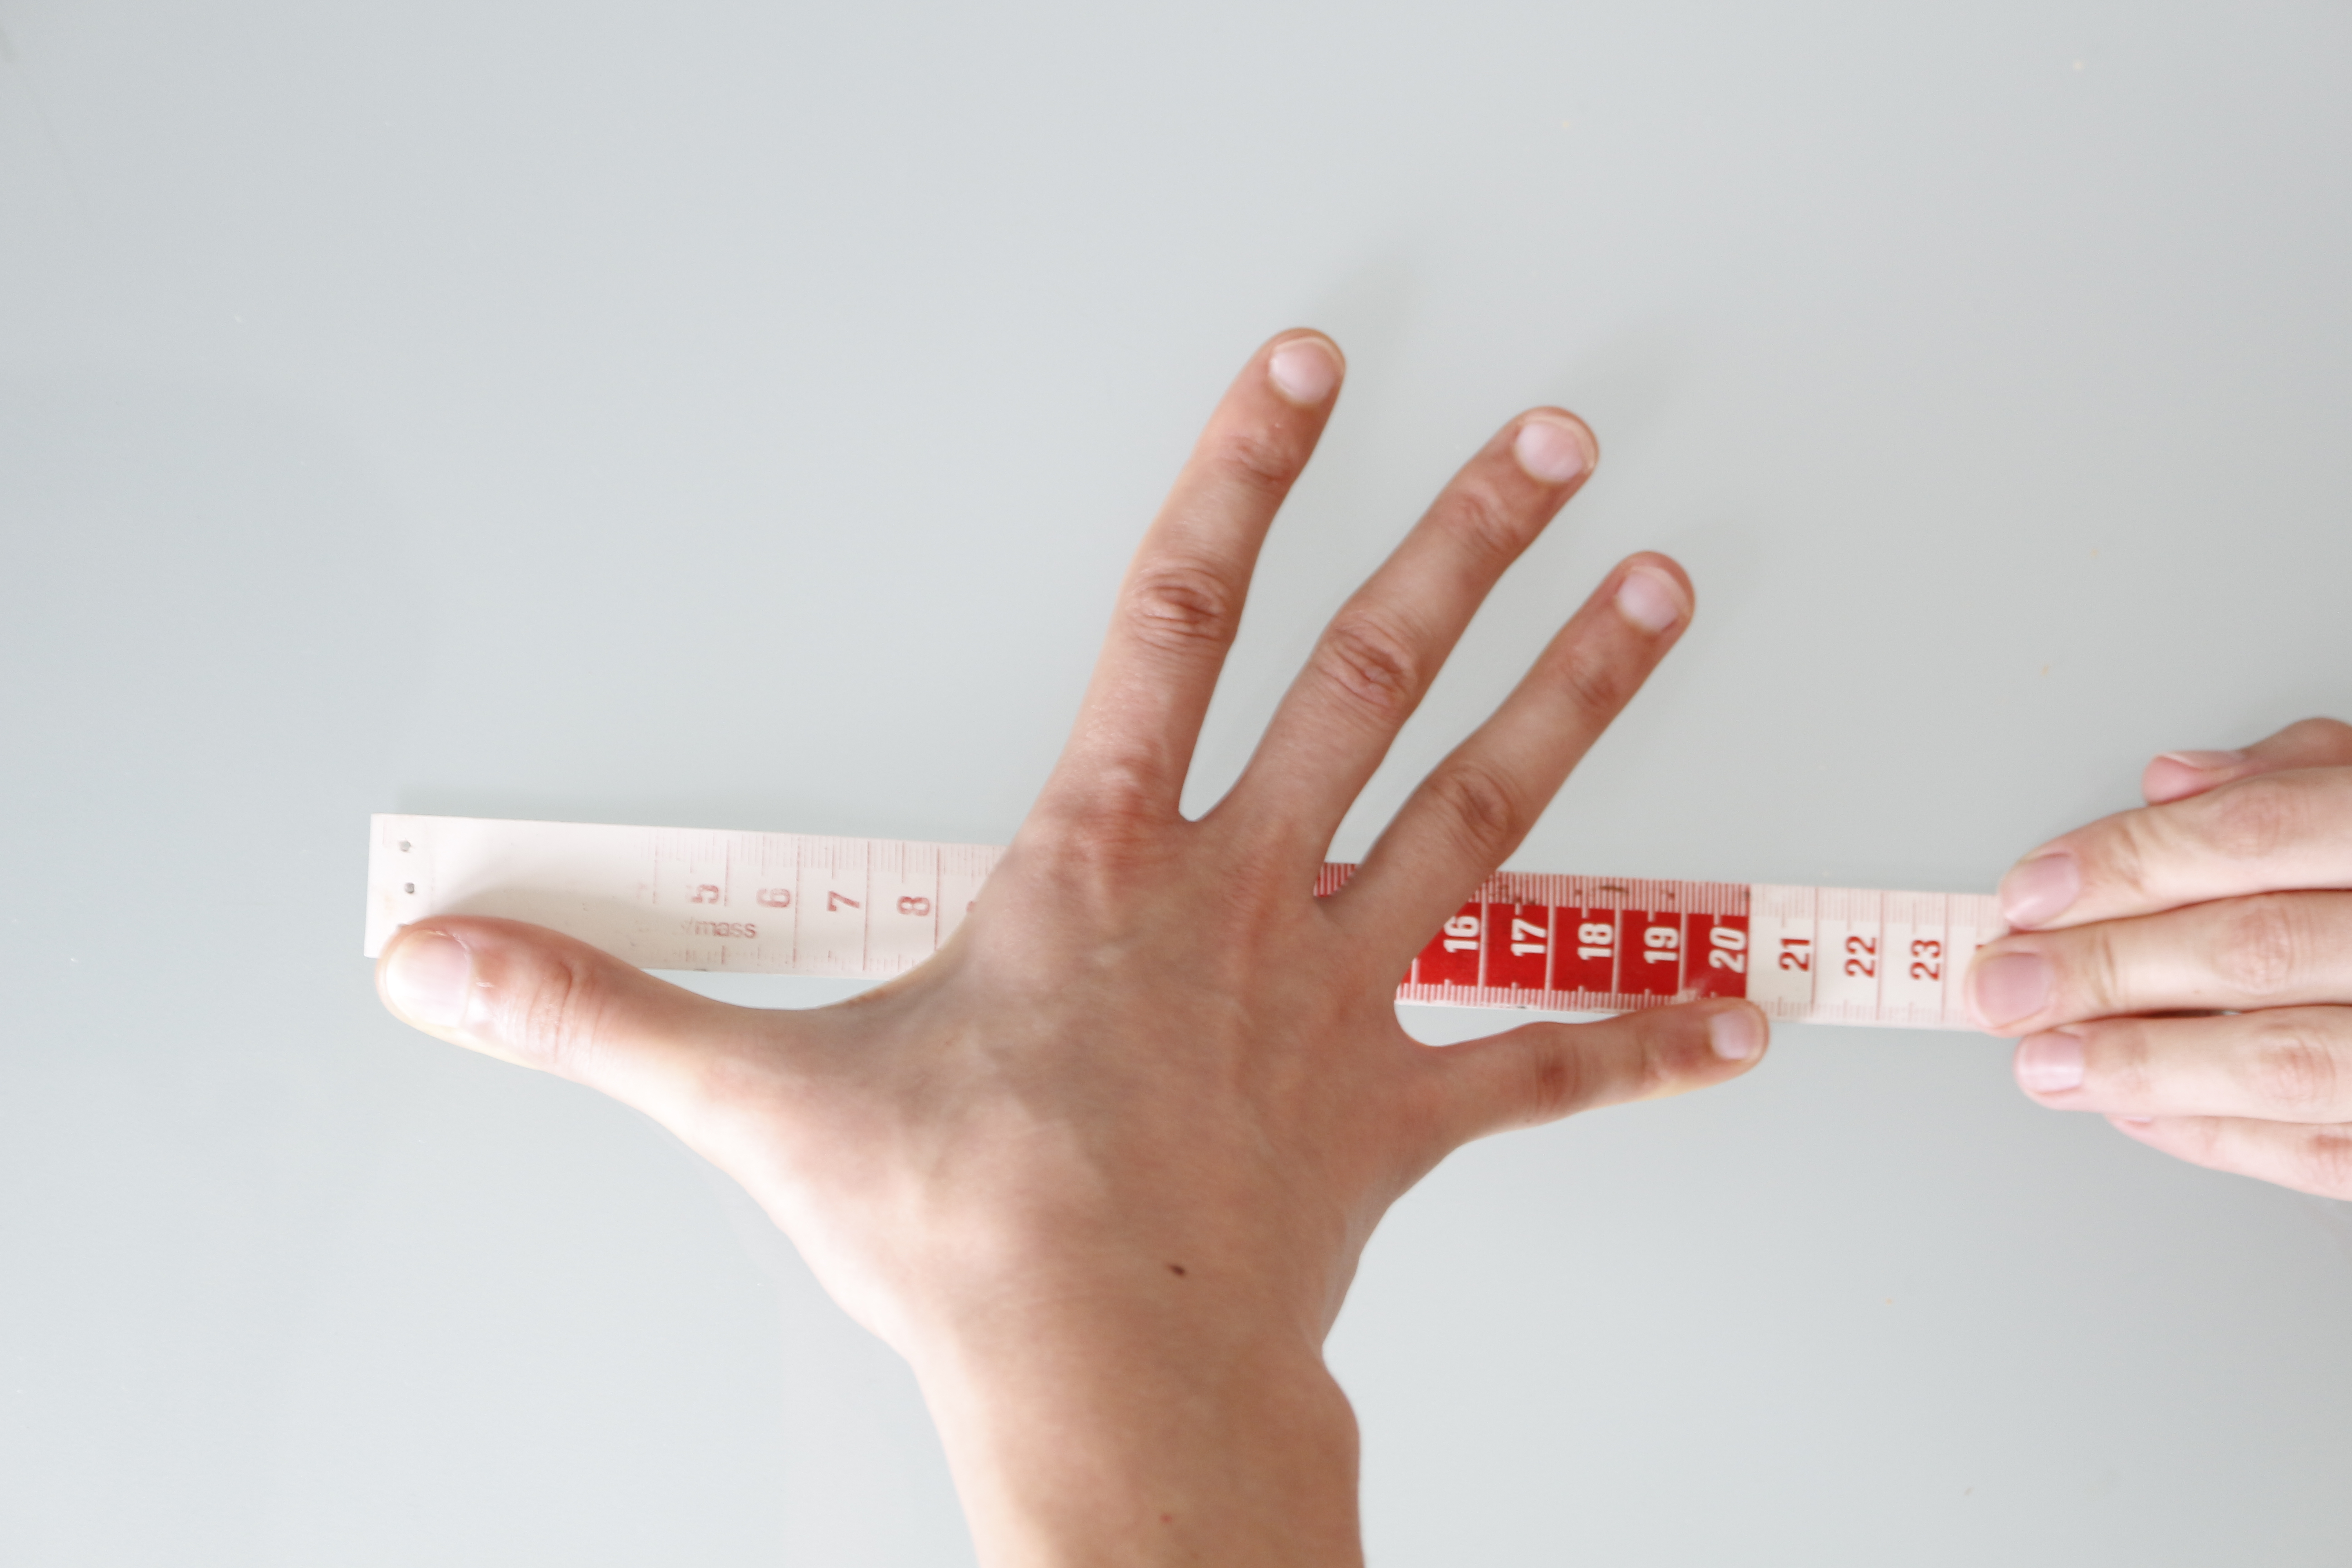
\includegraphics[width=0.24\textwidth]{figures/hand01}} 
    \subfigure[Hand Length]{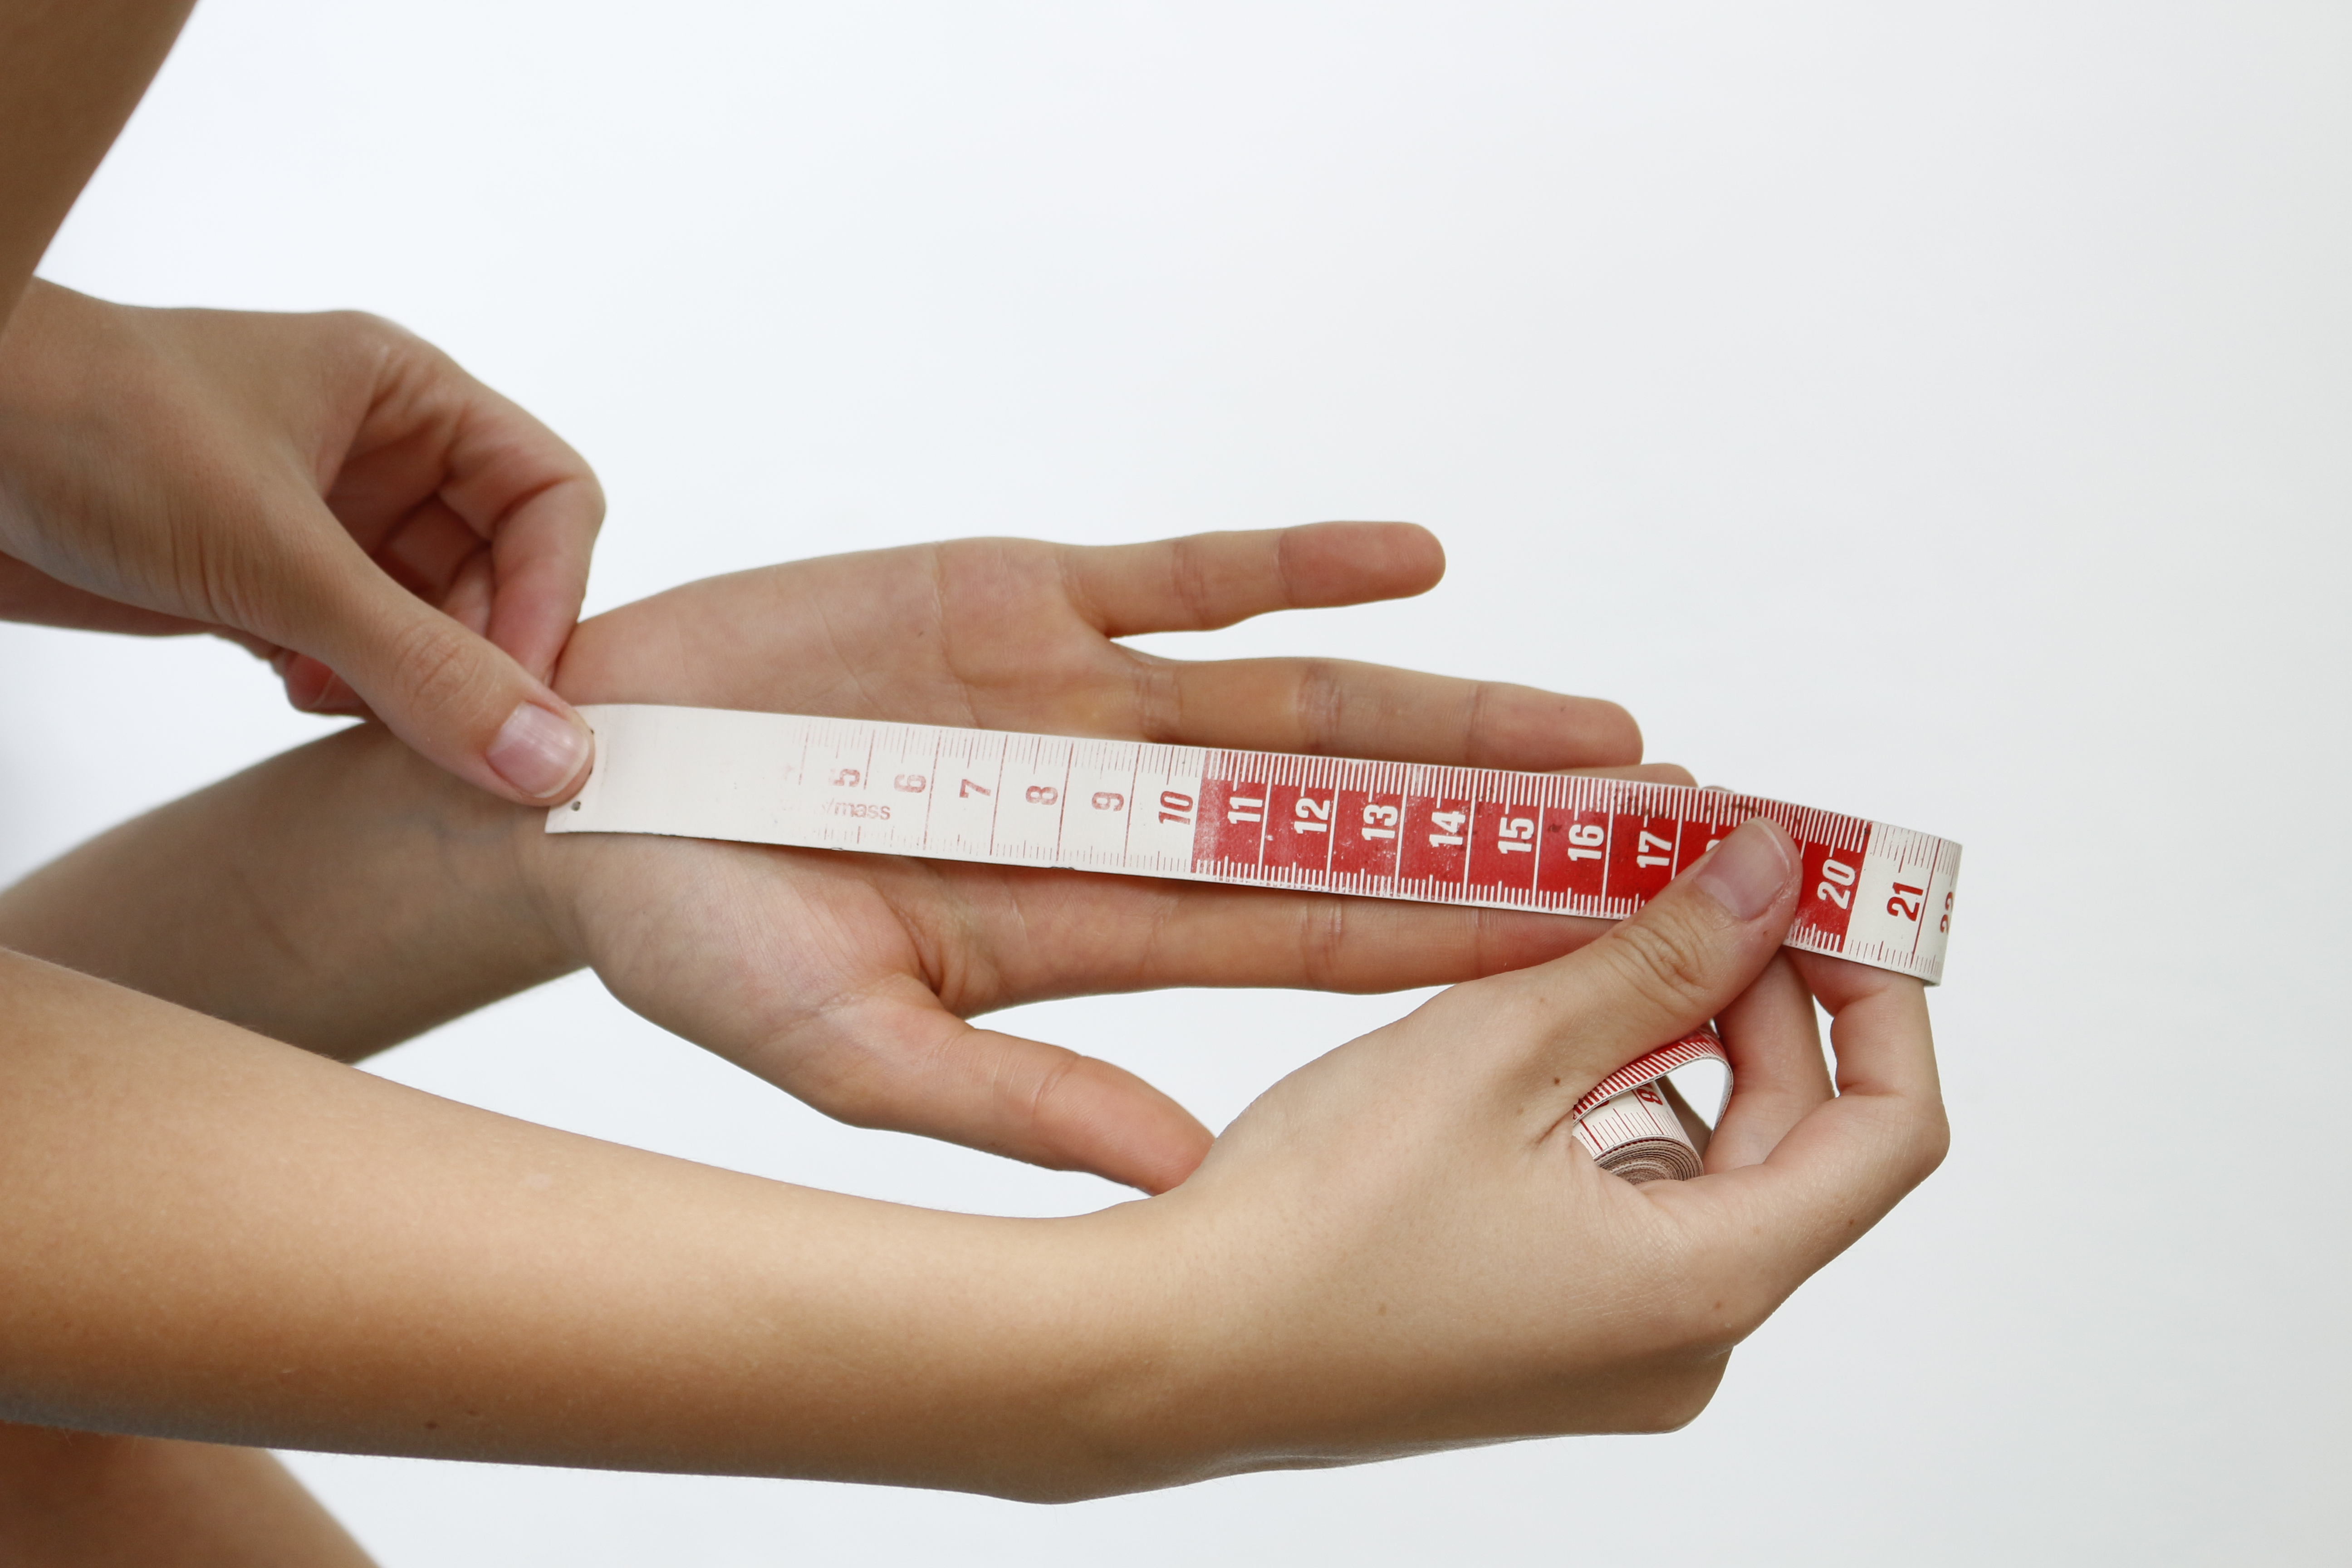
\includegraphics[width=0.24\textwidth, angle=90]{figures/hand02}} 
    \subfigure[Hand Width]{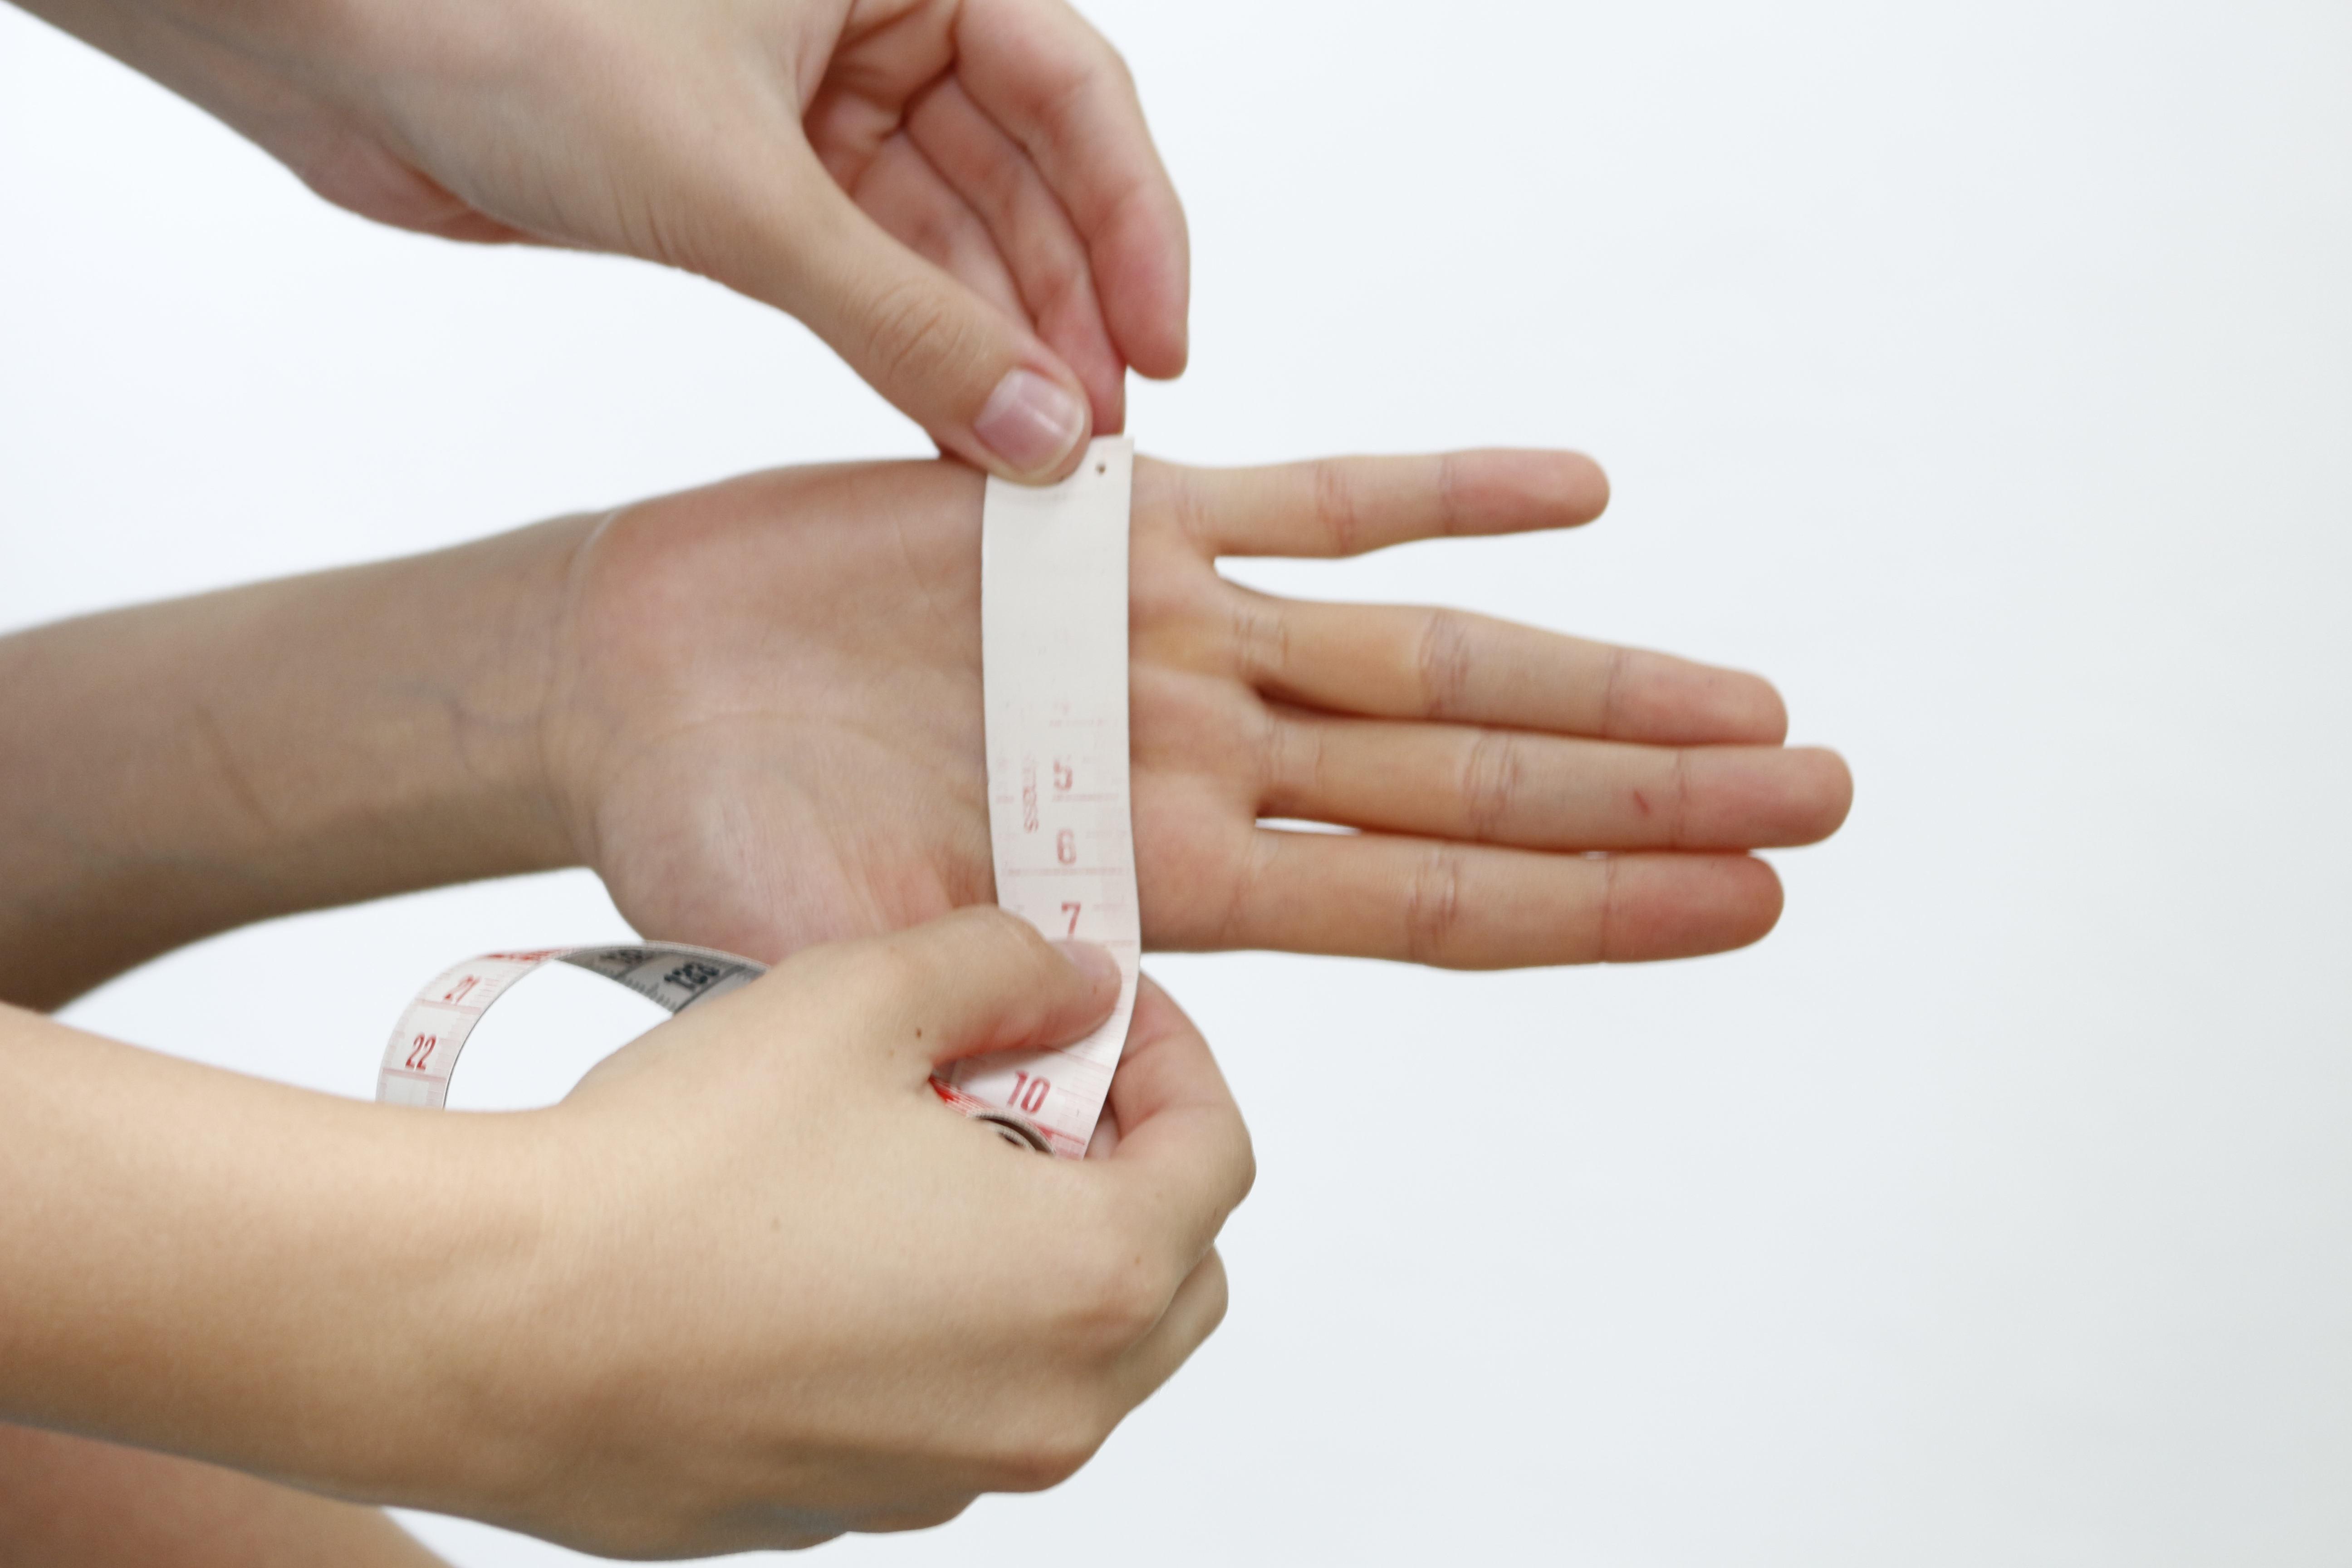
\includegraphics[width=0.24\textwidth, angle=90]{figures/hand03}} 
    \subfigure[Zomming Span]{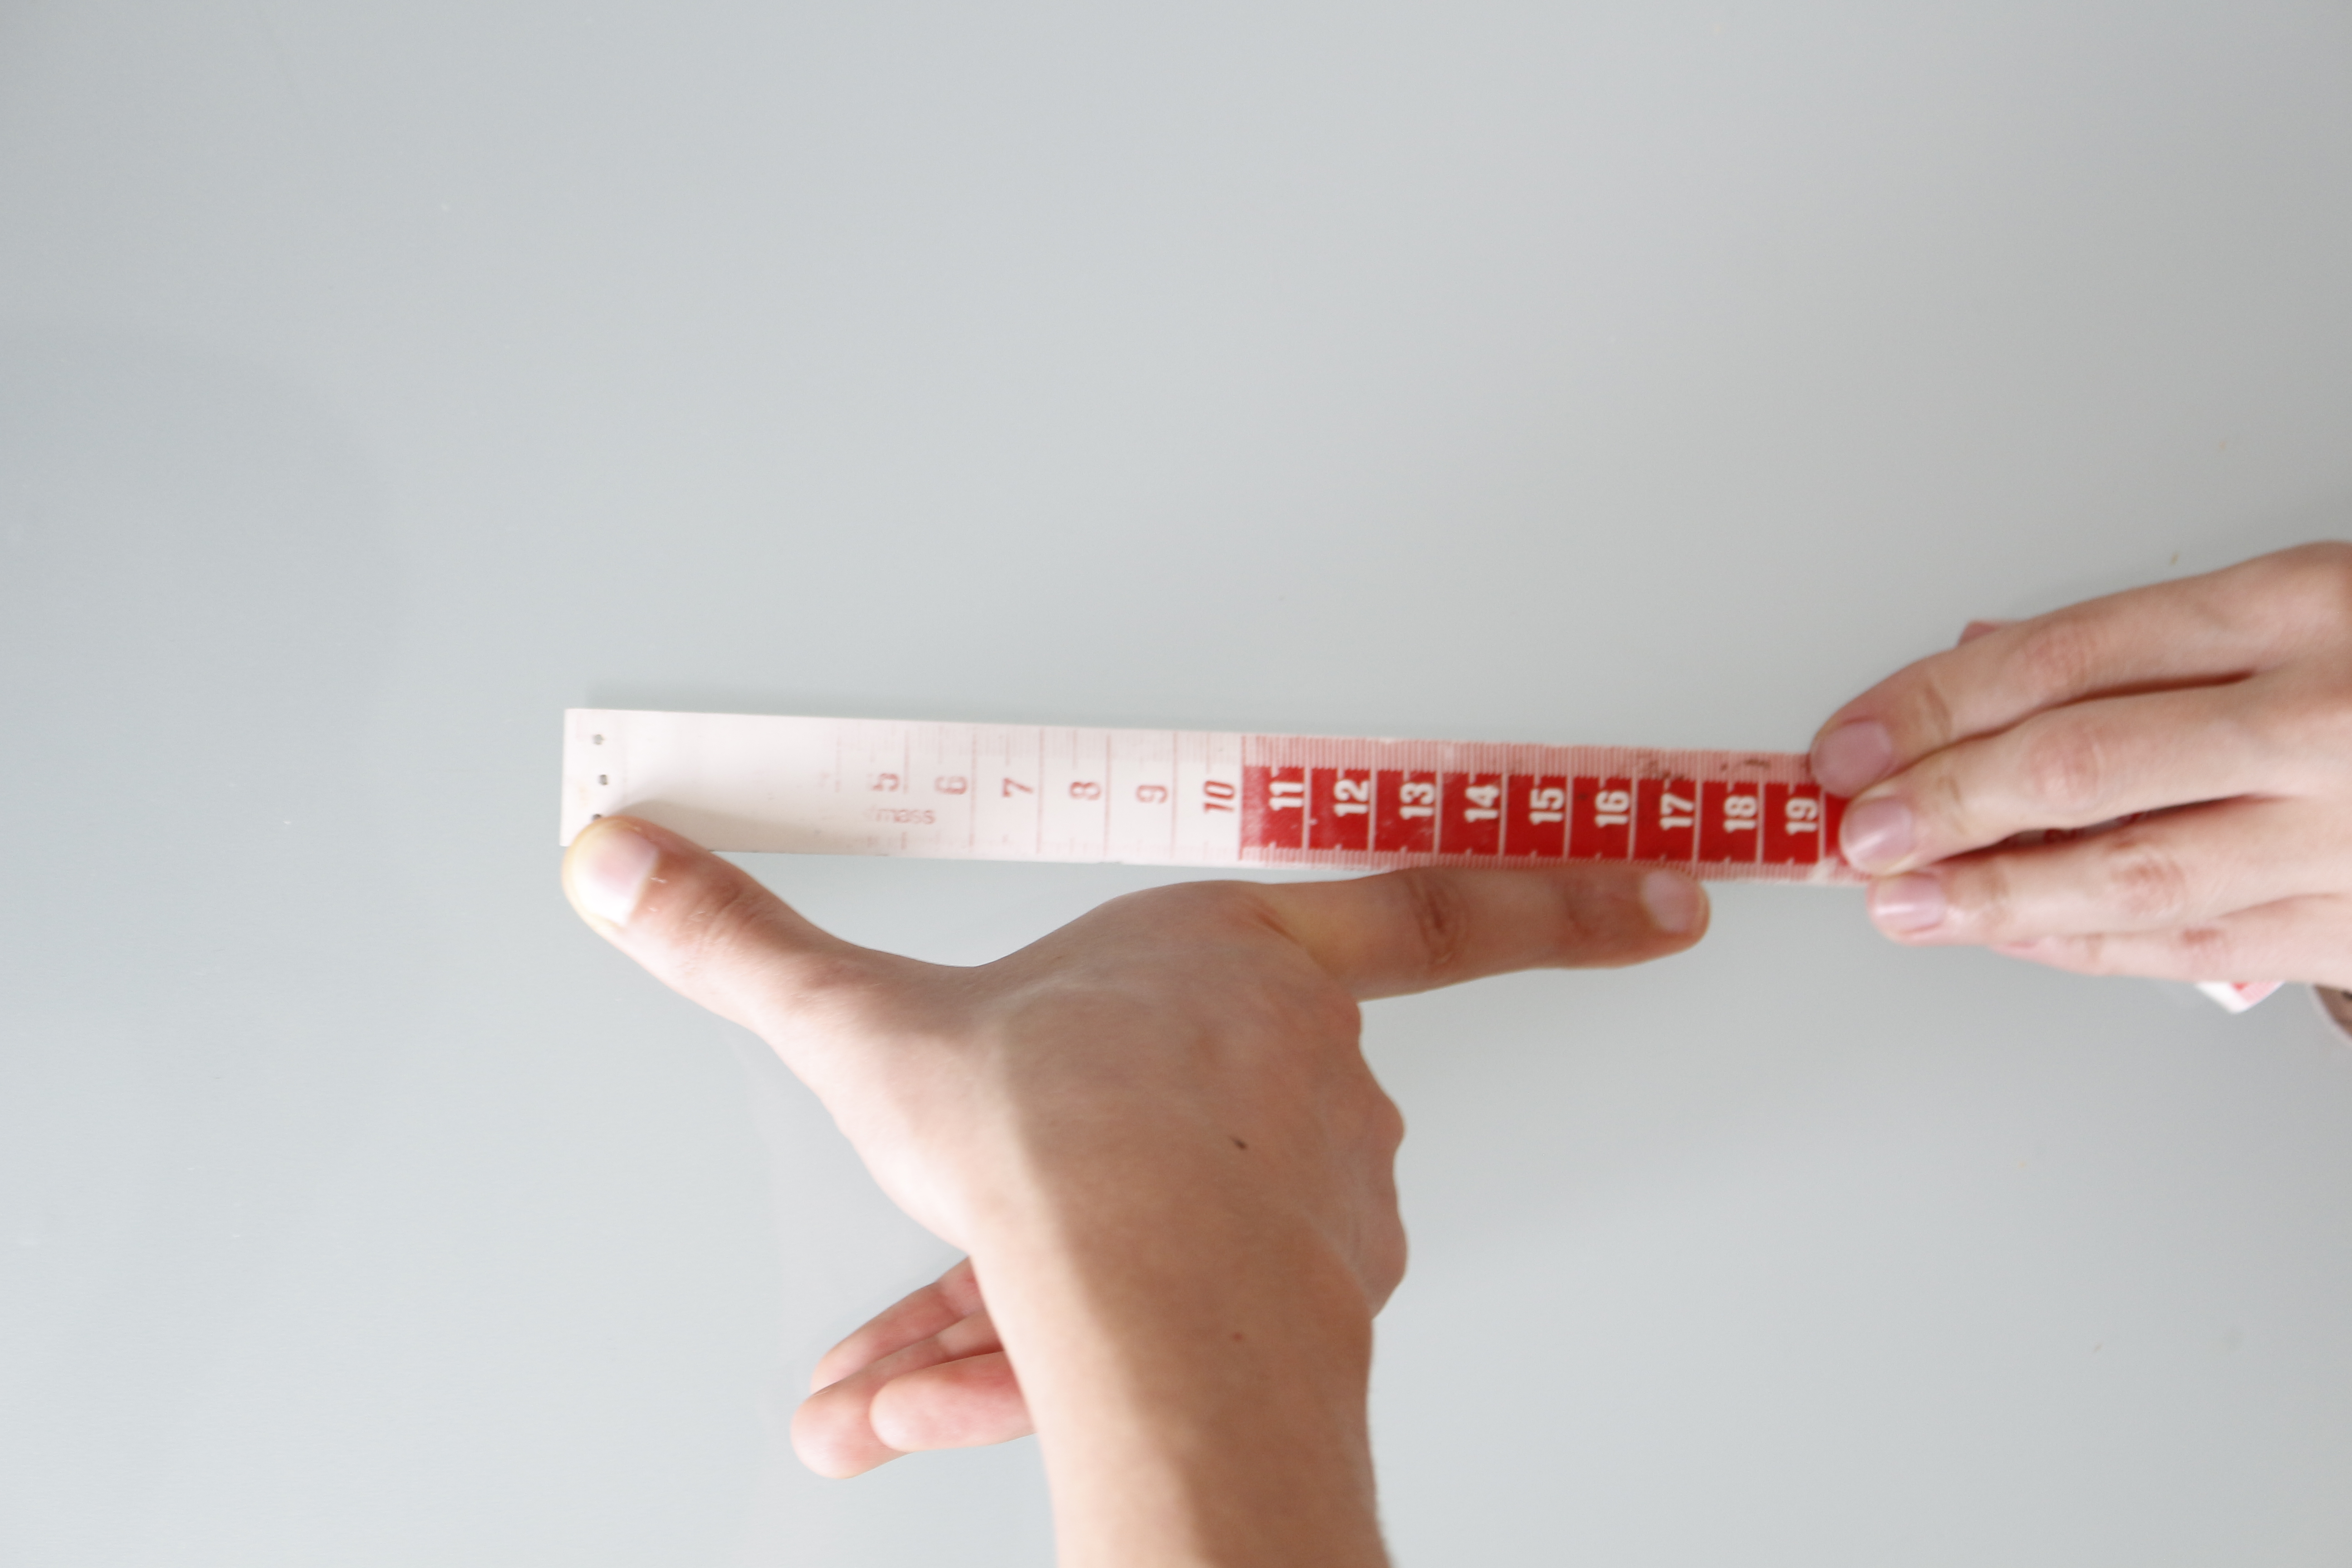
\includegraphics[width=0.24\textwidth]{figures/hand04}} 
\caption{Hand Measurements}
\end{figure*} 

\subsection{App}
The android application implemented for this study contained a screen for entering data about the user (hand measurements, age and gender). Before each task some instructions about the assignment were displayed. While performing the tasks, the application tracked different features which were stored into a database. These comprised of the x- and y- positions of the touch events and sensor data about acceleration, rotation and orientation. Task specific features were the number of scrolls, zooming span, timestamps etc.


\begin{figure*}
    \subfigure[Radius Task]{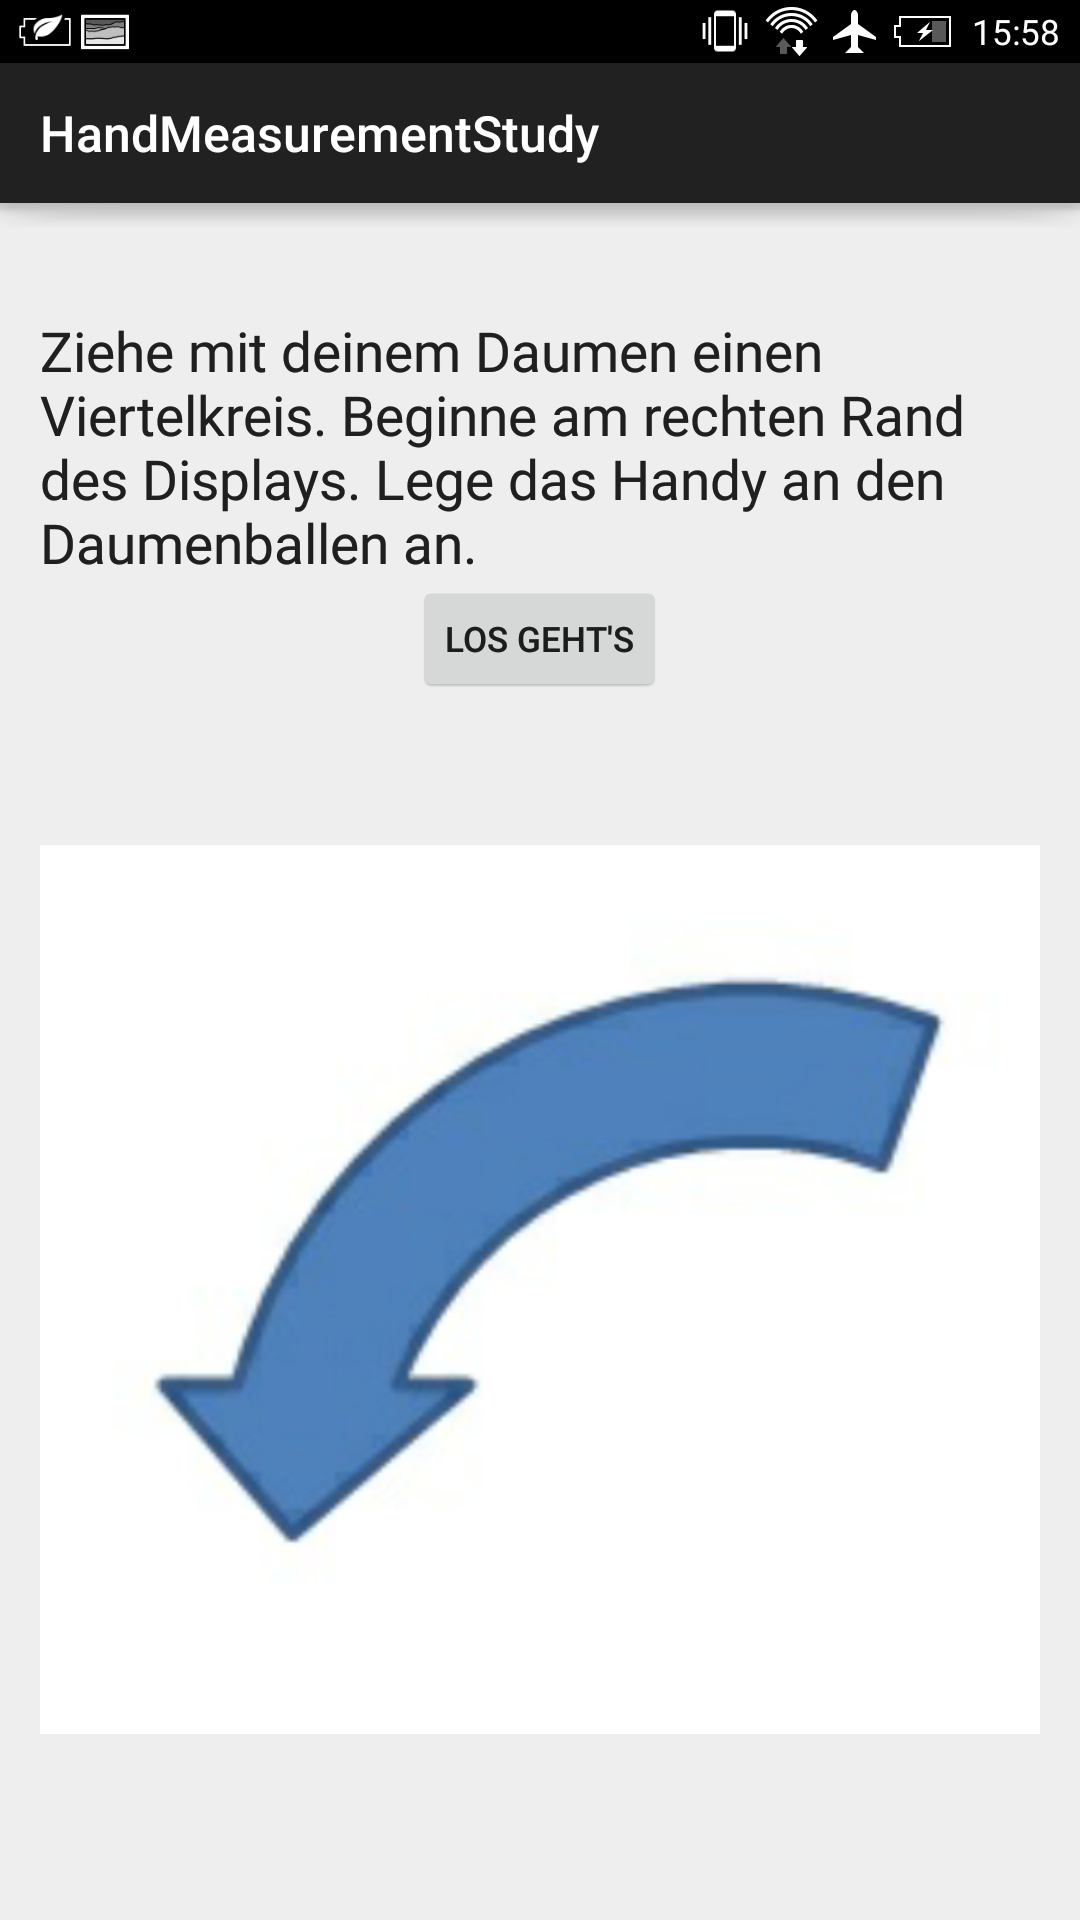
\includegraphics[width=0.16\textwidth]{figures/screenshot01.png}} 
    \subfigure[Tapping Task]{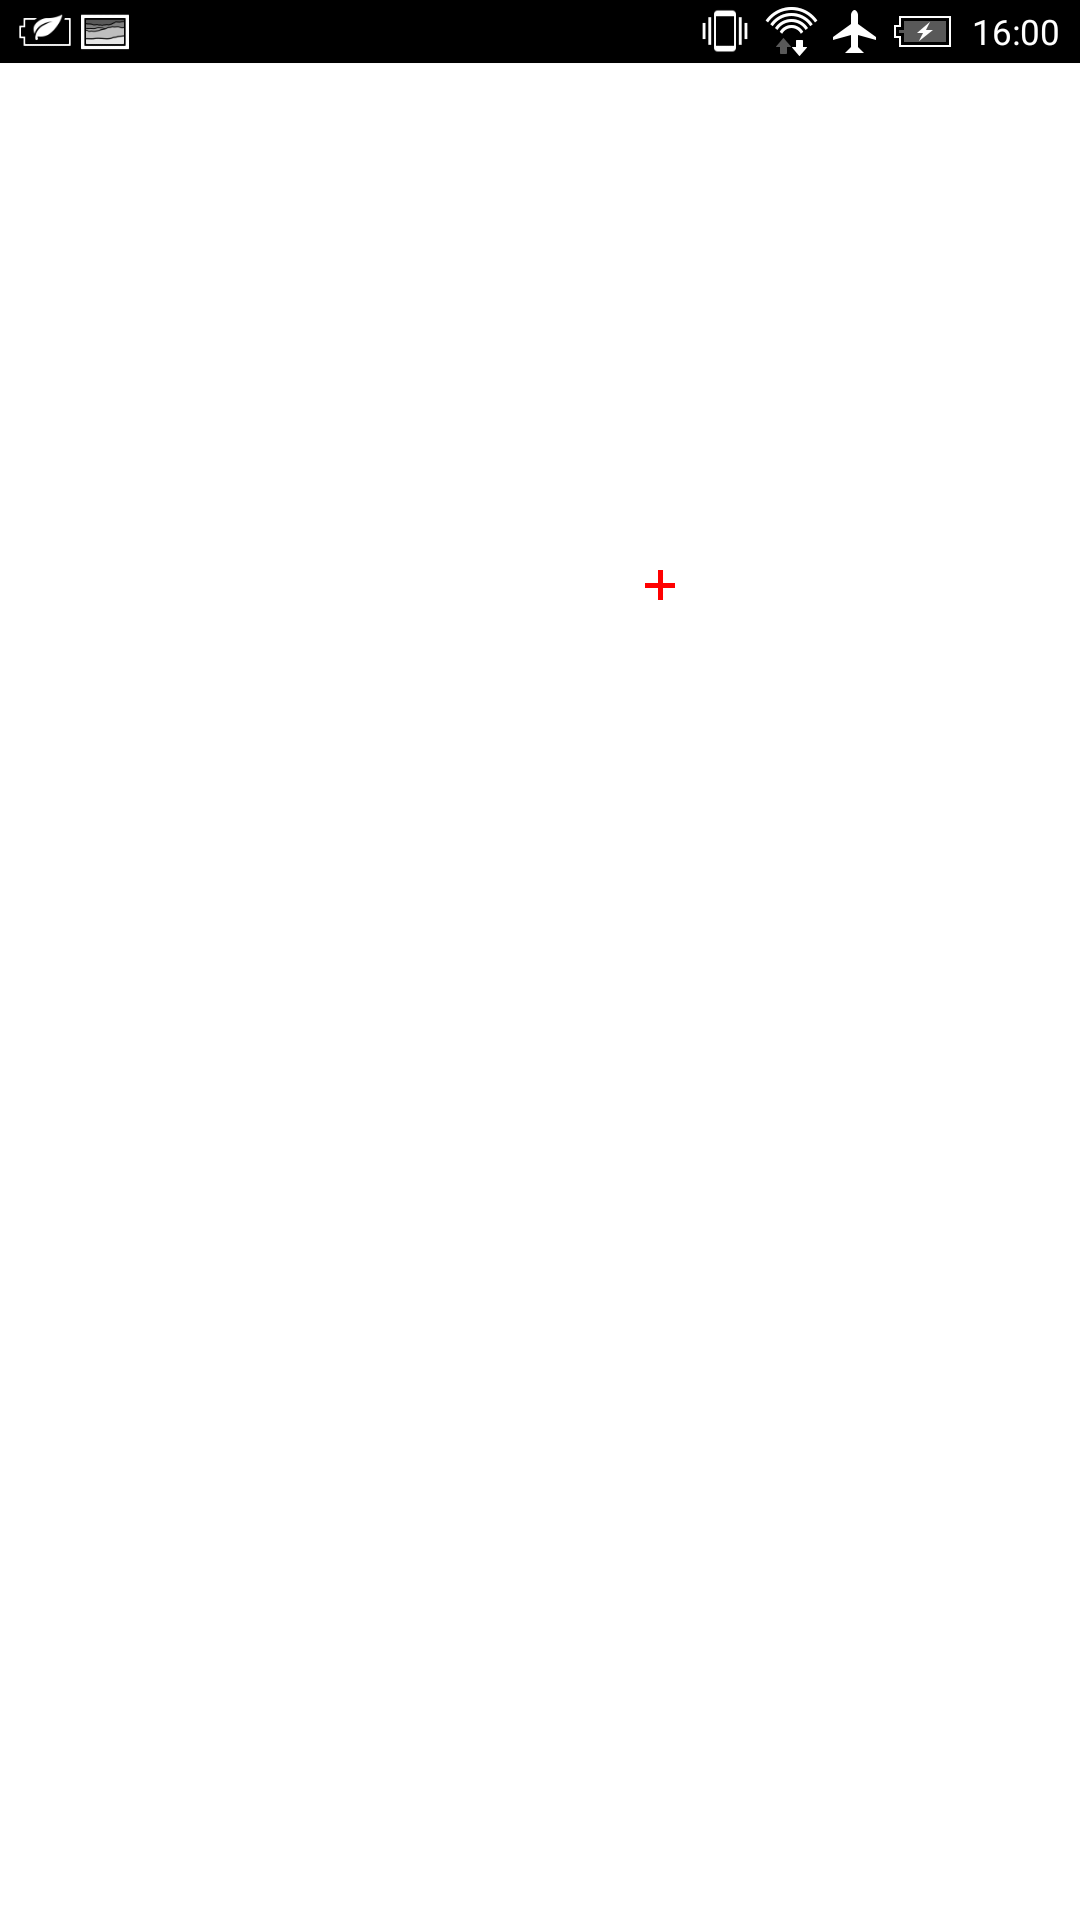
\includegraphics[width=0.16\textwidth]{figures/screenshot02.png}}
    \subfigure[Scrolling Task]{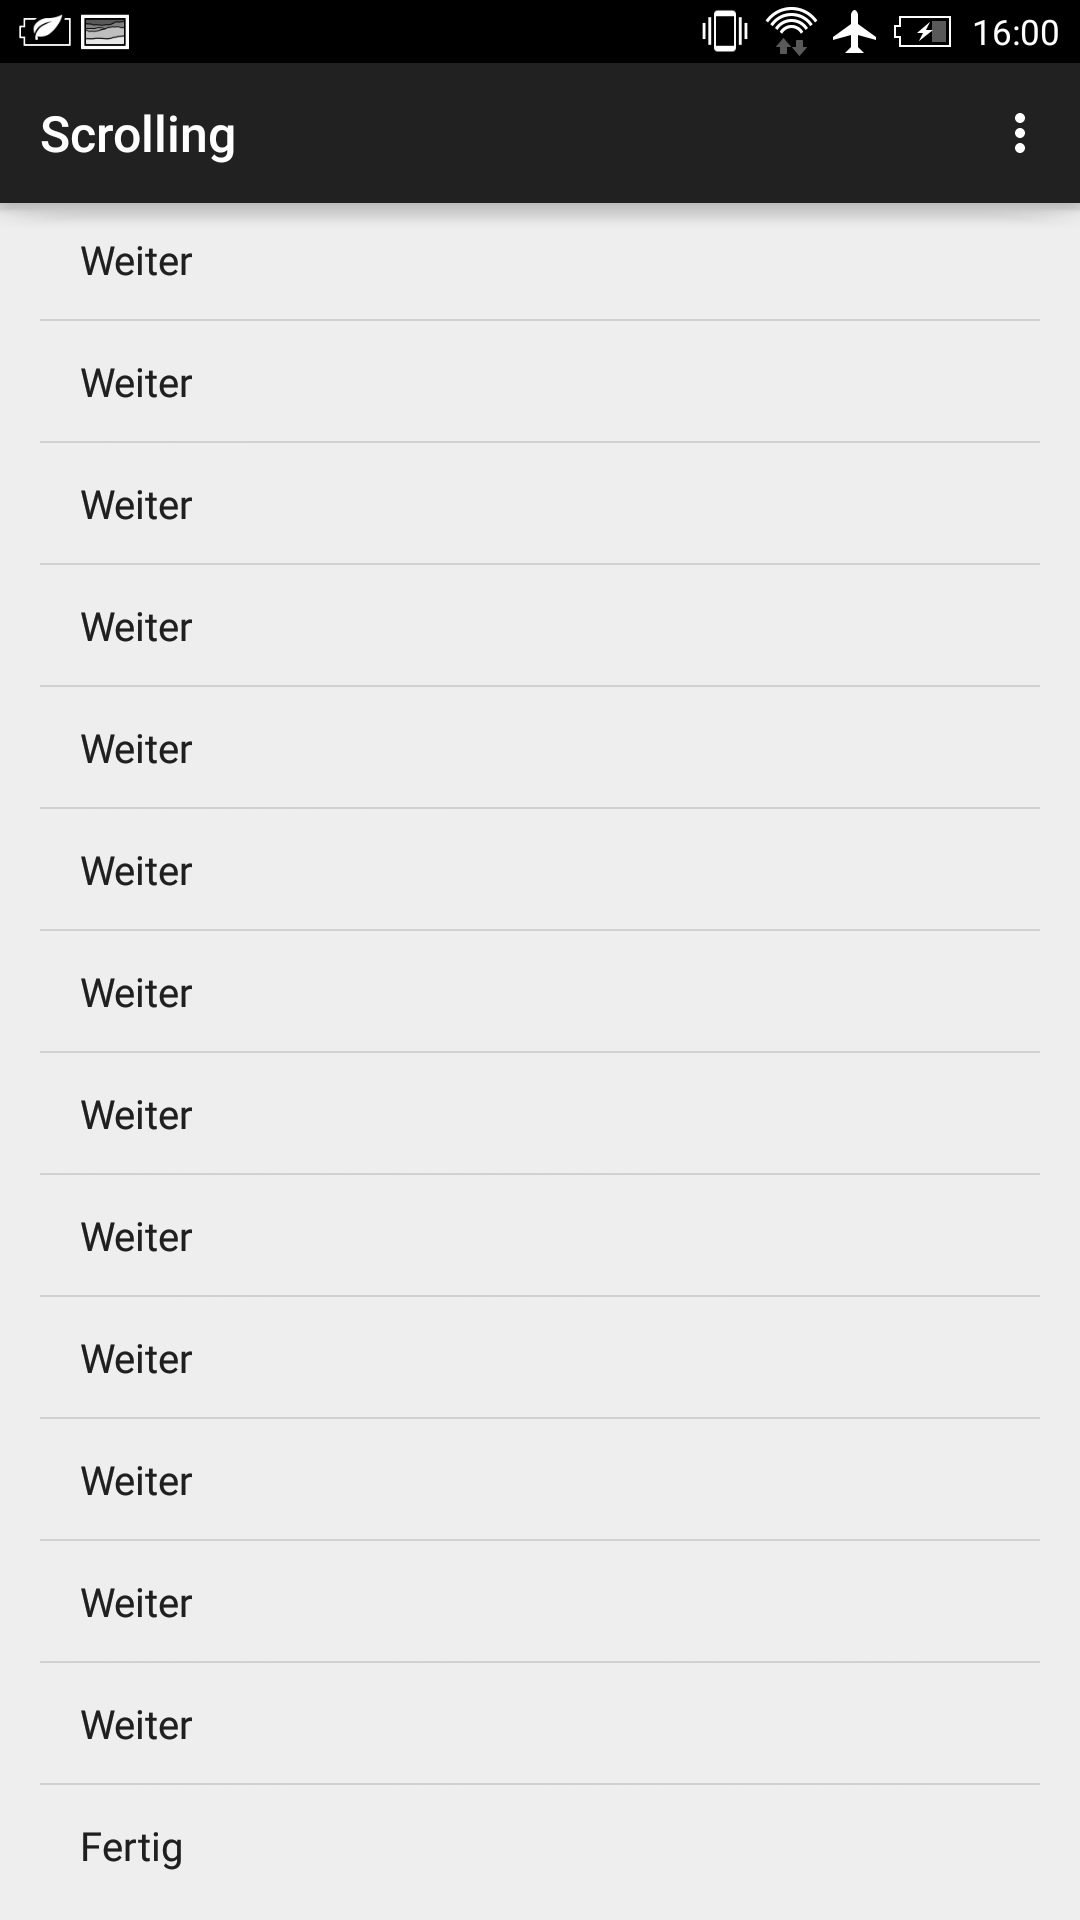
\includegraphics[width=0.16\textwidth]{figures/screenshot03.png}} 
    \subfigure[Swiping Task]{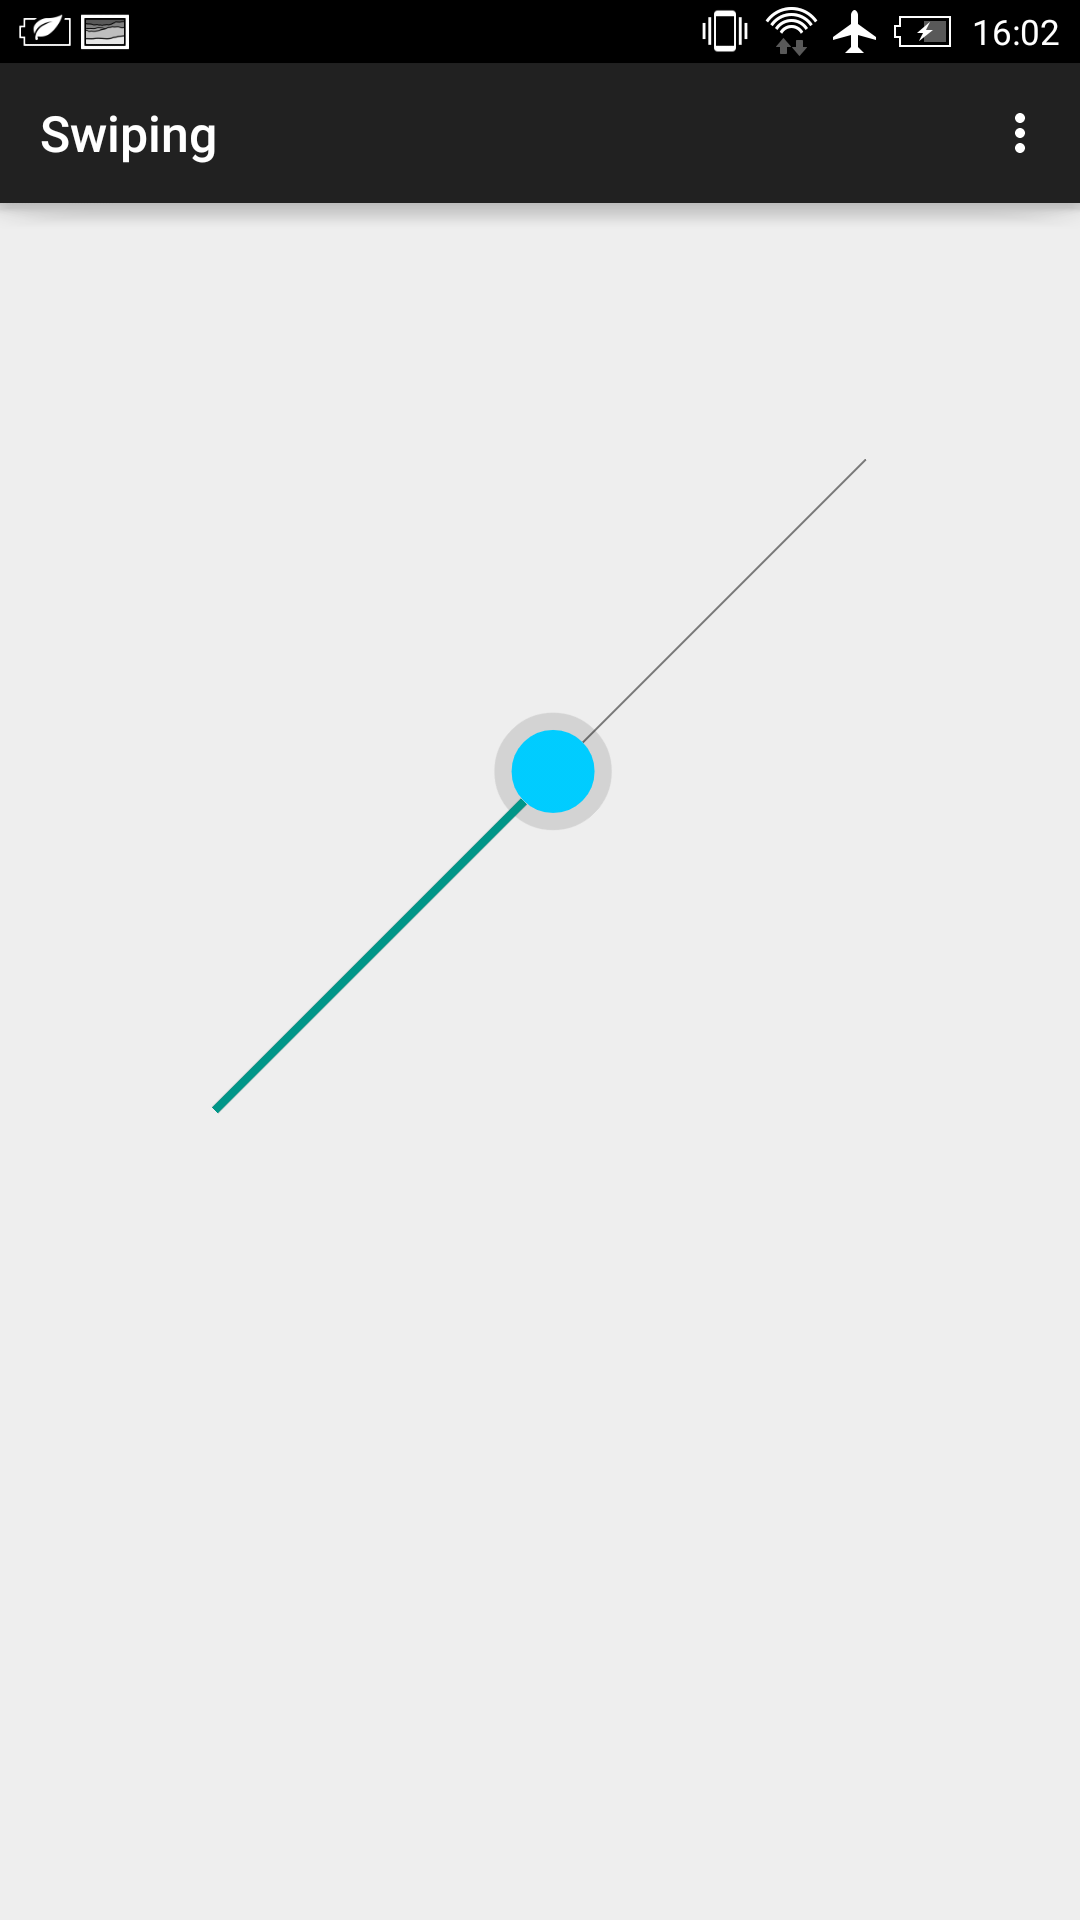
\includegraphics[width=0.16\textwidth]{figures/screenshot04.png}} 
    \subfigure[Maximum Zooming Task]{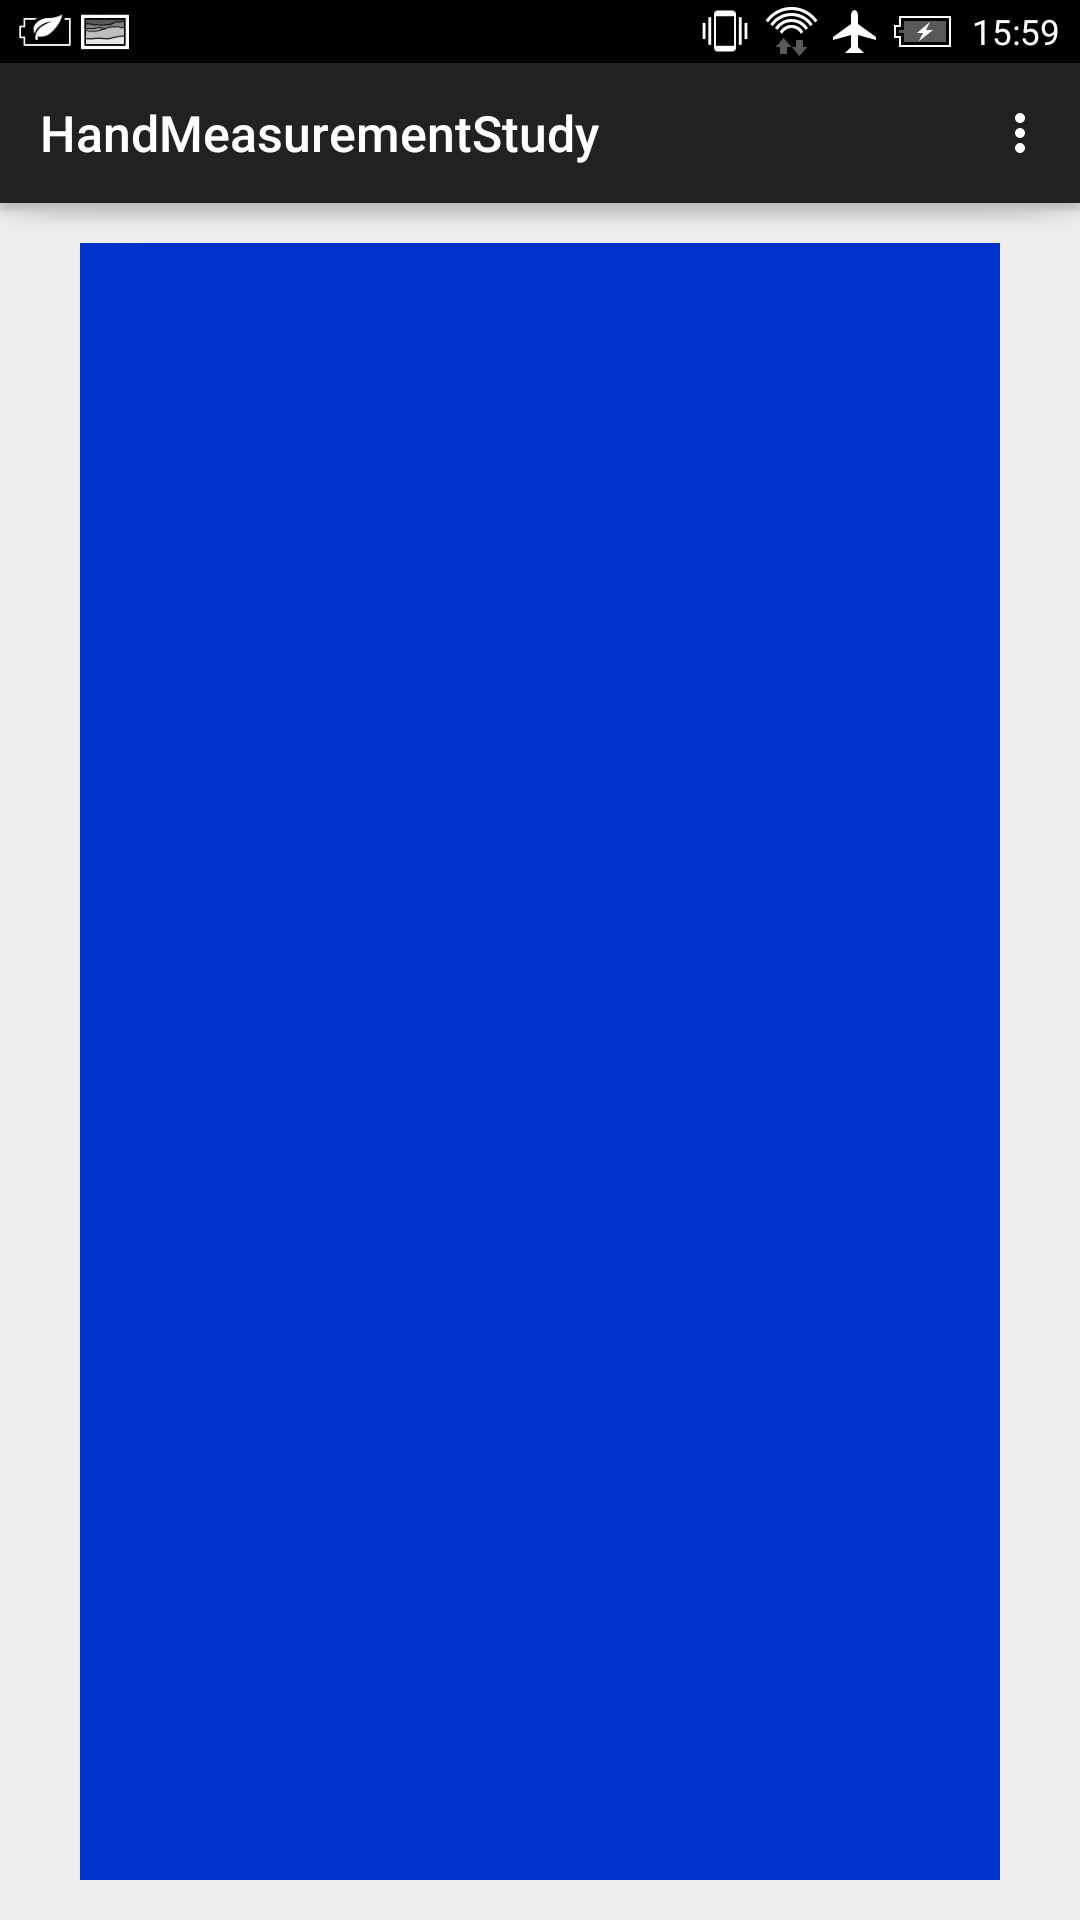
\includegraphics[width=0.16\textwidth]{figures/screenshot05.png}} 
    \subfigure[Frame Zooming Task]{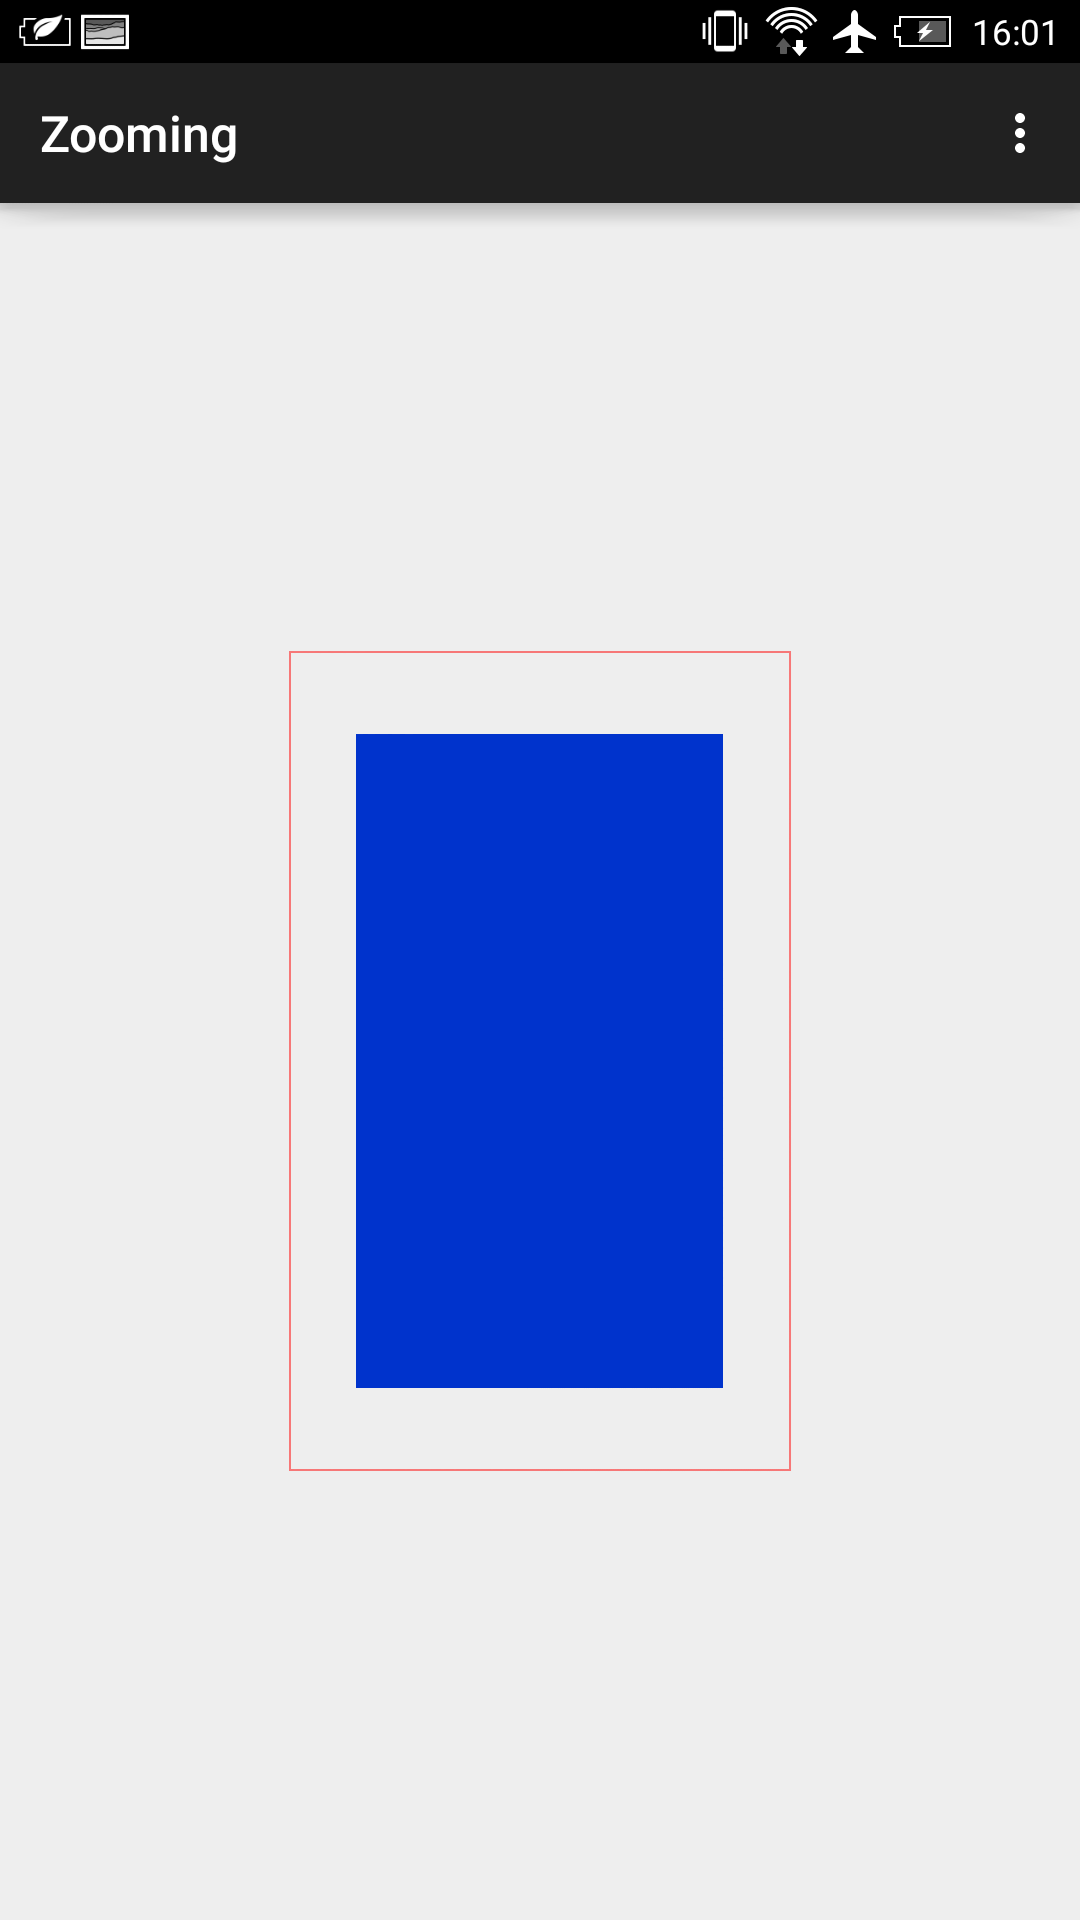
\includegraphics[width=0.16\textwidth]{figures/screenshot06.png}} 
\caption{Interaction tasks} 
\end{figure*} 


\subsection{Participants}
The 62 participants of this study were between 18 and 36 years old, 36 males and 26 females. Their hand lengths differed between 152 and 224 mm.

------------------Sarah ----------------------------------
\subsection{Procedure}
% Studienaufbau
The participants have been invited to a 15 minute time slot to take part in our hand measurement study. They could receive credits or an amazon voucher for their participation. In order to allow the usage of their hand and touch data, they had to sign a letter of agreement.\\
At first, the participants hand dimensions were measured manually as described before. Their data was then entered directly into our app. The participants started with the radius task in a predetermined hand position. After that, the tasks came up in a random order according to a latin square. The participants were free in solving the tasks, except they were only allowed to use one hand. For the zooming tasks, participants were instructed to use the other hand as well or to leave the device on the table.

------------------Jonas ----------------------------------\\
%\section{Evaluation}
=> was haben wir ausgewertet\\
"Signifikanz nicht untersucht, da nicht explorativ" !!!!! ... am interessantesten war dieses und jenes ... darauf eingehen => Plot zeigen und erläutern

\section{Results}
=> das korreliert mit xy
To understand the results of our study we first have to look at the measured hand data. The correlation of the different hand measurements is not as high as a naive assumption would suggest. The weaker correlations are with the total-span and with the zoom-span which is most likely caused by the measurement technique. For the zoom-span the subjects had to press their hand on the table and the span was measured. Some pressed stronger than others and others were physically able to spread their fingers wider. The tighter (?) measurements were therefore the with and the height of the hand, which also correlate more with 0.8x. Therefore we decided to compare the results with all four measurements separately (see table \ref{handSizeCorrelations}).
\begin{itemize}
\item results overview
\item detailed analysis of high correlations with plots (according to presentation)
\end{itemize}


\begin{table}[]
\centering
\caption{Hand size correlations}
\label{handSizeCorrelations}
\begin{tabular}{ll|llll}
 &users  &total span  &zoom span  &length  &width  \\ \hline
 &total span  &  &0.74  &0.705  &0.754 \\
 &zoom span  &0.764  &  &0.772  &0.669 \\
 &length  &0.702  &0.757  &  &0.818 \\
 &width  &0.776  &0.673  &0.841  &
\end{tabular}
\end{table}


\section{Discussion}

------------------Sarah ----------------------------------
\section{Conclusion and Future Work}
We came up with different challenges when investigating hand size and mobile touch interactions. In our study, it was hardly possible to determine the user's hand size from his mobile touch interactions during our tasks.\\
We could show a higher correlation between touch interaction and hand size when we determined the hand position. As this might be uncomfortable for users, the other tasks in our study were designed in such a way that hand position is free and left over to the user.\\
Further investigations should eventually determine hand positions in order to evaluate the user's hand size. As the most promising result we got was from our radius task, this could eventually be used to predict the user's hand size.\\ 
%hier nochmal results zusammen fassen
Knowing about the user's hand size could then enhance mobile interaction. If our mobile devices know about our hand sizes, they could adapt the user interfaces in order to facilitate the interaction. Navigation bars and other important UI Elements could be moved to make them more reachable.


\begin{itemize}
\item Conclusion: am vielversprechendsten ist vermutlich ... Wie würde man speziell dieses noch in neuer Studie untersuchen
\item weitere Daten angucken und evaluieren
\item make mobile interaction smarter (Bezug zur Introduction nehmen)
\end{itemize}



% Balancing columns in a ref list is a bit of a pain because you
% either use a hack like flushend or balance, or manually insert
% a column break.  http://www.tex.ac.uk/cgi-bin/texfaq2html?label=balance
% multicols doesn't work because we're already in two-column mode,
% and flushend isn't awesome, so I choose balance.  See this
% for more info: http://cs.brown.edu/system/software/latex/doc/balance.pdf
%
% Note that in a perfect world balance wants to be in the first
% column of the last page.
%
% If balance doesn't work for you, you can remove that and
% hard-code a column break into the bbl file right before you
% submit:
%
% http://stackoverflow.com/questions/2149854/how-to-manually-equalize-columns-
% in-an-ieee-paper-if-using-bibtex
%
% Or, just remove \balance and give up on balancing the last page.
%
\balance{}


% BALANCE COLUMNS
\balance{}

% REFERENCES FORMAT
% References must be the same font size as other body text.
\bibliographystyle{SIGCHI-Reference-Format}
\bibliography{literature}

\end{document}

%%% Local Variables:
%%% mode: latex
%%% TeX-master: t
%%% End:
